\documentclass[../Hovedrapport.tex]{subfiles}
\begin{document}

\chapter{Software og styring}
    \label{sec:Software og styring}
I det følgende afsnit vil softwaren og styringen for systemet blive gennemgået. Disse aspekter er en essentiel del af kølesystemet og sørger for at systemet fungerer, som det er tiltænkt. Softwaren vil i det følgende blive gennemgået, således der opnås en forståelse for, hvordan denne skal betjenes og en evt. ny bruger kan benytte kølesystemet. Brugerfladen vil blive gennemgået, så der opnås en forståelse for, hvordan der manøvreres rundt i denne. Det vil ikke blive gennemgået, hvad der sker bag denne brugerflade i form af blockdiagrammer og anden programmering. Foruden dette vil styringen af kompressoren og blæserne blive gennemgået senere.

% Den nedestående section er til Marcus.

\section{Software (B.B. \& M.N.)}
Til styringen af systemet er fire programmer blevet udarbejdet: 
\begin{itemize}
    \item Kalibreringsprogram til trykmåler
    \item Kalibreringsprogram til temperaturmåler
    \item Loginprogram
    \item Styringsprogram
\end{itemize}
De fire programmer virker som ét stort program med fire individuelle funktioner. Når programmet startes, vil en loginside blive åbnet. Dette har til funktion at sikre den fremtidige dataintegritet. Derudover kontrollerer programmet også om den person, der logger ind, er administrator eller ej. Dette gøres, da administratorer har adgang til flere funktioner end almindelige brugere.
Det er f.eks. kun administratorer, som kan tilgå de forskellige kalibrerinsprogrammer samt oprette nye brugere.
%------------------------------------------------------------------------------
\subsection*{Grafisk brugerflade}
    \label{sec:grafisk_bruger}
Den grafiske brugerflade er udviklet med fokus på brugervenlighed, og vil blive beskrevet mere dybdegående i de følgende underafsnit.
%------------------------------------------------------------------------------
\subsection*{Loginside}
Det første brugeren ser, når denne starter programmet, er et loginvindue. Her er der mulighed for at logge ind med en allerede kendt konto i systemet. Der bliver her påkrævet et brugernavn og password. Når disse er indtastet, kan der trykkes på 'Login'-knappen, og hvis de indtastede oplysninger er korrekte, vil brugeren blive sendt videre i programmet.\\
Hvis brugeren har glemt sit password, kan der trykkes på knappen: 'Glemt kode', hvilket vil anmode brugeren om dennes e-mailadresse, hvormed kodeordet vil blive fremsendt.

Funktionen samt designet fremgår af nedenstående figur.
\begin{figure}[H]
	\centering
	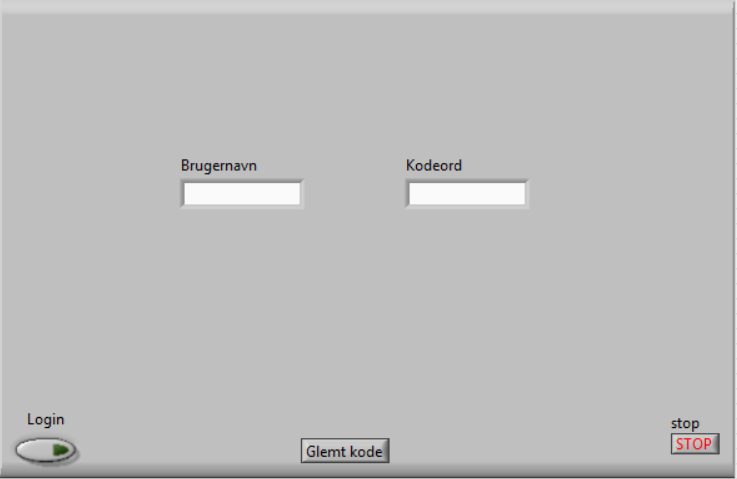
\includegraphics[width=0.80\textwidth]{Billeder/login.png}
	\caption{\textit{Loginfane}.}
	\label{fig:login}
\end{figure}
\begin{figure}[H]
	\centering
	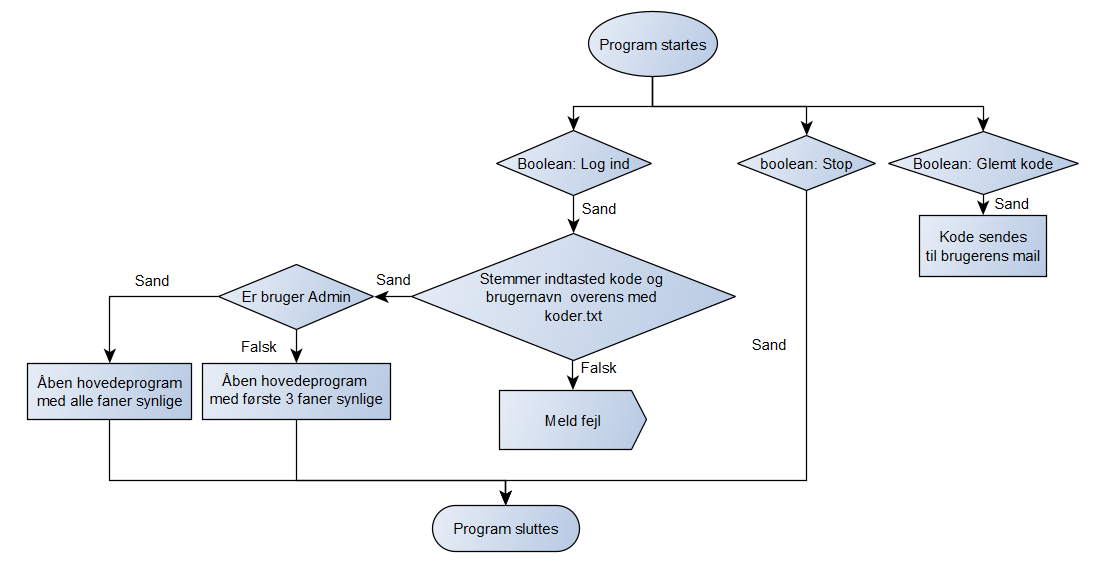
\includegraphics[width=0.80\textwidth]{Billeder/login_vi.png}
	\caption{\textit{Loginfane funktion}.}
	\label{fig:login}
\end{figure}
%------------------------------------------------------------------------------
\subsection*{Oversigt}
Det første, der møder brugeren, når der er blevet logget ind, er et vindue, hvor den ønskede temperatur i systemet kan indstilles. Dette betyder, at systemet vil indregulere sig efter den ønskede temperatur, hvilket gøres ved hjælp af en PID-regulering. Reguleringen har til formål gradvist at indstille kompressorens omdrejningstal, så en on/off-regulering undgås så vidt muligt. Når kompressorens omdrejningstal ikke kan blive mindre, vil denne slukke, så der ikke bliver for koldt i køleskabet. Desuden er der i dette vindue mulighed for at skifte mellem de andre fire faner, logge af samt se hvorvidt systemet er tændt. Når systemet bliver kølet, vil der i højre side forekomme et symbol i form af et snefnug, som lyser blåt. Når kompressoren er slukket, vil det i stedet være gråt (se figur \ref{fig:oversigt}).\\
Oppe i det højre hjørne er en dropdown menu, hvor brugeren kan vælge hvilken DAQ, der skal bruges til tryk- og temperaturmålinger. Hvis DAQ'en ikke stemmer overens med det, som computeren navngiver den, vil programmet lukke ned og give en fejlmeddelelse nede i venstre hjørne.
Der vil nederst i venstre hjørne også være en hilsen til brugeren, der er logget ind, hvori der står 'Velkommen [Bruger]' . Til højre for denne hilsen, er en knap, hvor brugeren kan logge ud. Slutteligt er der en 'Stop'-knap, som stopper programmet.
\begin{figure}[H]
	\centering
	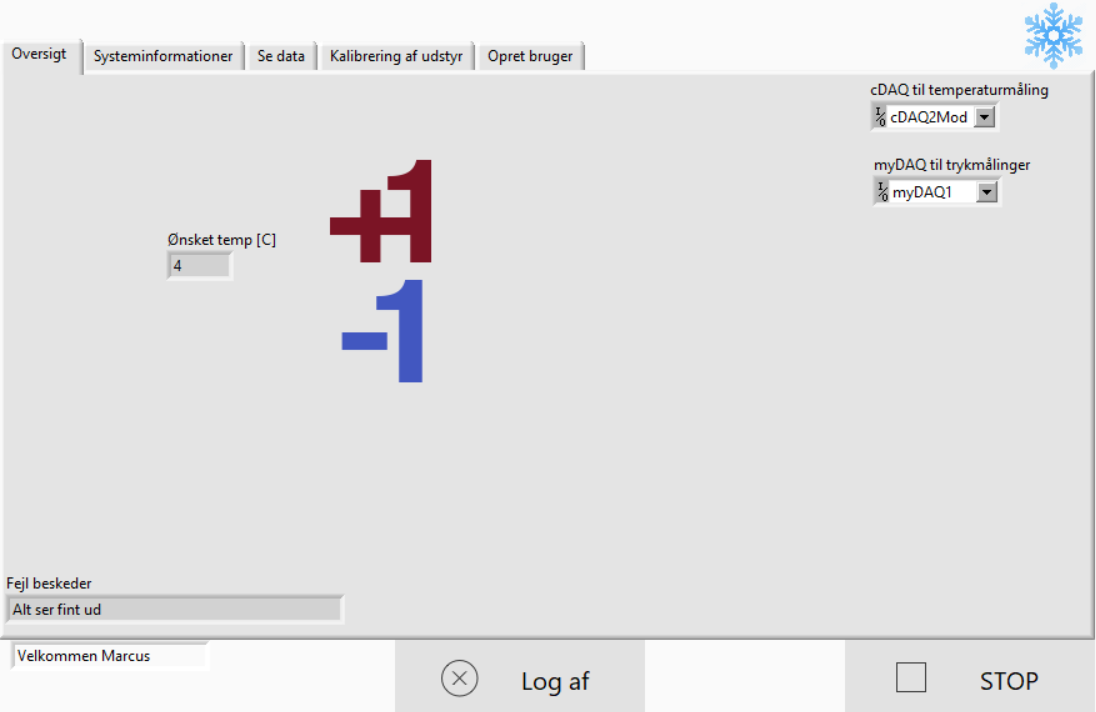
\includegraphics[width=0.80\textwidth]{Billeder/oversigt.png}
	\caption{\textit{Temperaturindstilling}.}
	\label{fig:oversigt}
\end{figure}
%------------------------------------------------------------------------------
\subsection*{Systeminformation}
I fanen 'Systeminformation' kan systemet startes ved den øverste knap til venstre ved navn 'Tænd/sluk anlæg', hvormed køleskabet startes.
Det skal dog bemærkes, at for at kompressoren kan starte, skal modstanden også være aktiveret, hvilket gøres med knappen 'aktiver modstand'.
Under denne knap møder brugeren en ny knap, der hedder 'Start målinger', hvor brugeren har mulighed for starte logning af forskellige målte samt udregnede data. Yderst til højre på brugerfladen fremgår fire bokse ved navn 'Sensor'. Disse sensorer er ikke navngivet ligesom de øvrige sensorer i fanen 'Se data', da disse er flytbare. 
\begin{figure}[H]
	\centering
	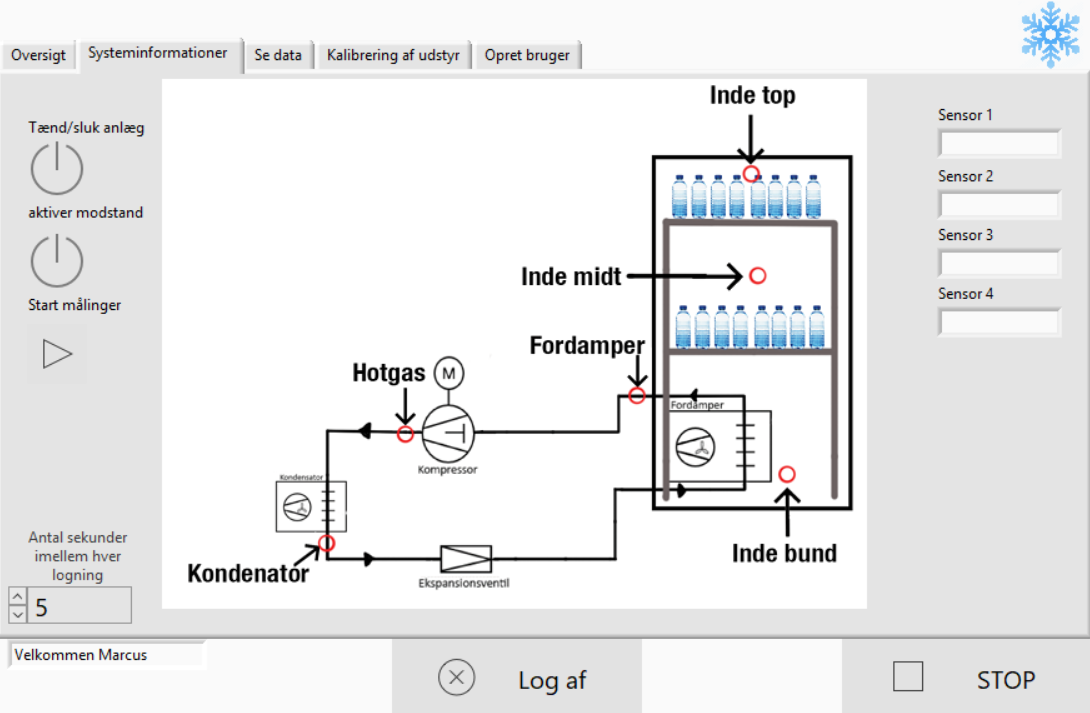
\includegraphics[width=0.80\textwidth]{Billeder/systeminfo.png}
	\caption{\textit{Systeminformationsfane}.}
	\label{fig:systeminformation}
\end{figure}
\vspace{-0.3cm}
%------------------------------------------------------------------------------
\subsection*{Se data}
Ved valg af fanen 'Se data' kan brugeren se forskellige temperaturer i systemet, når programmet kører. Den første temperatur, der måles, er temperaturen efter fordamperen. Derefter måles hotgastemperaturen efter kompressoren samt temperaturen efter kondensatoren. Disse tre målinger er de eneste temperaturer, som måler på kølemidlet. Foruden disse måles temperaturen også tre steder inde i køleskabet. Disse temperaturer måles i henholdsvis bunden, midten og toppen, hvorpå der udregnes et gennemsnit af disse temperaturer, der plottes som grafen til venstre. Derudover måles trykket også på det køletekniske systems højtryks- og lavtrykside.\\
I de målte temperaturer og tryk er der taget stilling til nøjagtigheden af målingerne, hvilket er angivet med en usikkerhed.
\begin{figure}[H]
	\centering
	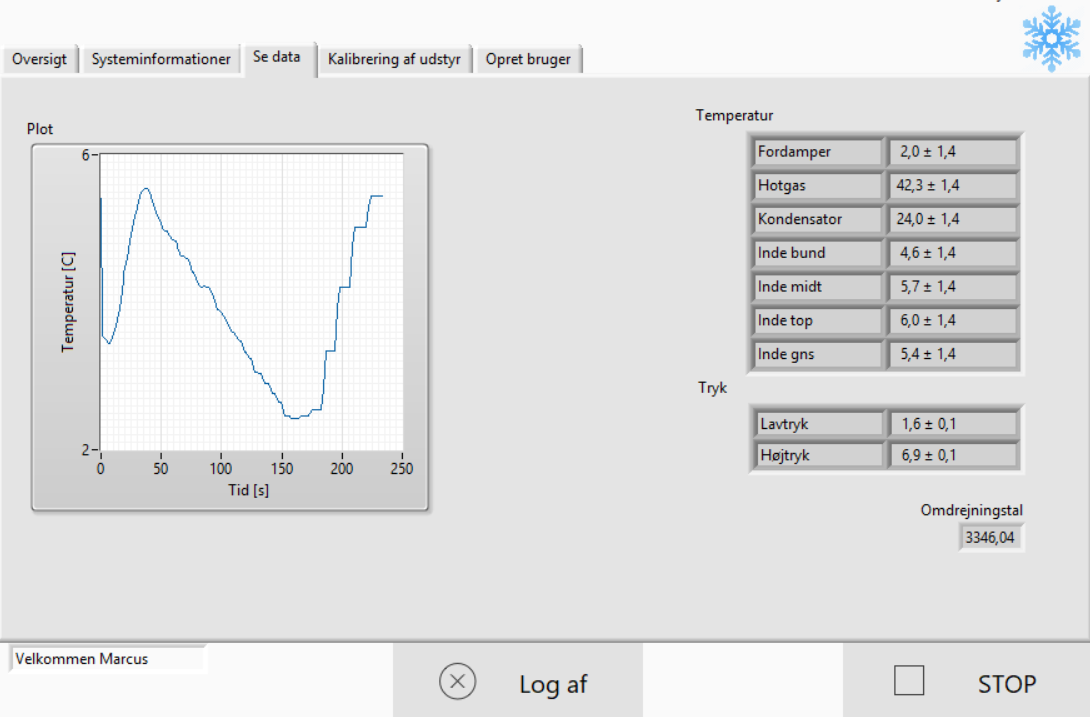
\includegraphics[width=0.80\textwidth]{Billeder/se_data.png}
	\caption{\textit{Se data}.}
	\label{fig:se_data}
\end{figure}
%------------------------------------------------------------------------------
\subsection*{Kalibrering af udstyr}
I den fjerde fane er der mulighed for at kalibrere thermocouples og trykmålere. Dette fungerer ved, at der trykkes på enten knappen 'Kalibrering af thermocoupler' eller knappen 'Kalibrering af trykmåler'. Ved at vælge en af disse knapper åbner et nyt program, som giver mulighed for at kalibrere disse sensorer. \\
Når der trykkes på knappen 'Opdater usikkerheder', vil brugeren blive anmodet om at indskrive de nye usikkerheder for temperaturer og tryk.\\
Slutteligt kan det nederst på siden til højre vælges, hvor stor indflydelse de forskellige led i PID-reguleringen skal have på omdrejningstallet.
Det skal bemærkes, at denne fane kun er synlig, hvis brugeren er administrator.
\begin{figure}[H]
	\centering
	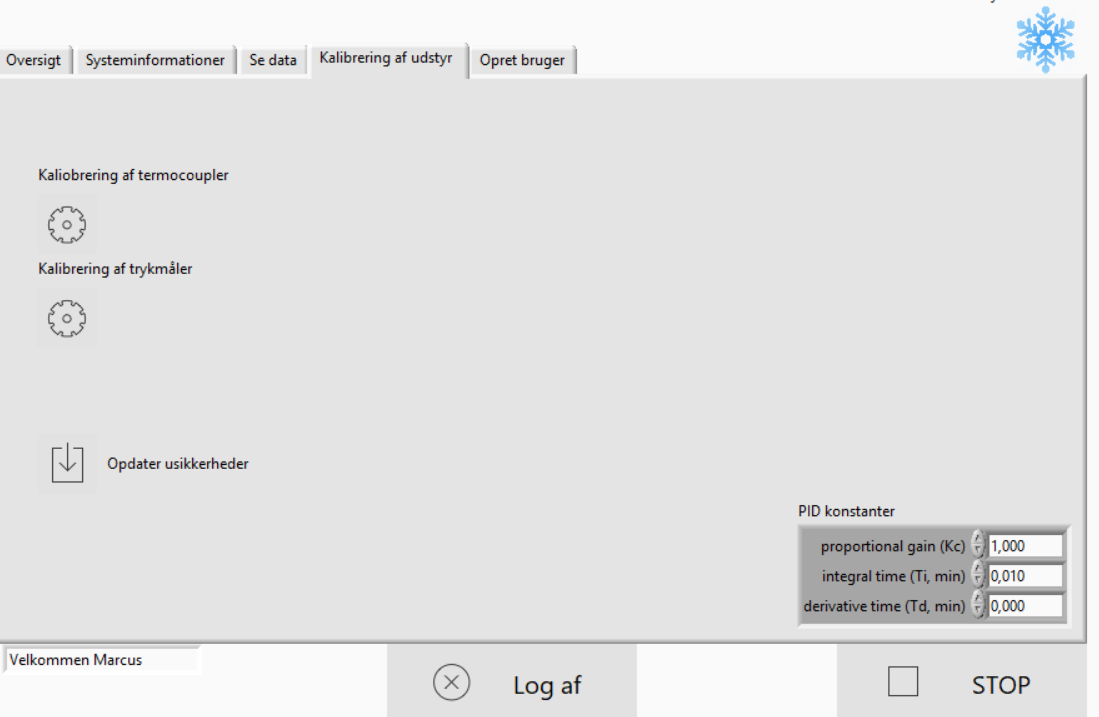
\includegraphics[width=0.80\textwidth]{Billeder/kali.png}
	\caption{\textit{Kalibreringsfane}.}
	\label{fig:kalibrering}
\end{figure}
%------------------------------------------------------------------------------
\subsection*{Opret bruger}
I denne fane kan en administrator oprette en ny bruger og angive en status på denne. Brugeren skal her angive et navn, et ønsket brugernavn, en kode samt bekræfte denne og slutteligt angive sin e-mailadresse, hvormed et glemt password kan fremsendes. Når dette er foretaget, kan knappen 'Opret bruger' benyttes til at oprette brugeren. Hvis denne bruger allerede er oprettet, vil vedkommende, som forsøger at oprette en bruger, blive anmodet om at finde på et andet brugernavn. 
\begin{figure}[H]
	\centering
	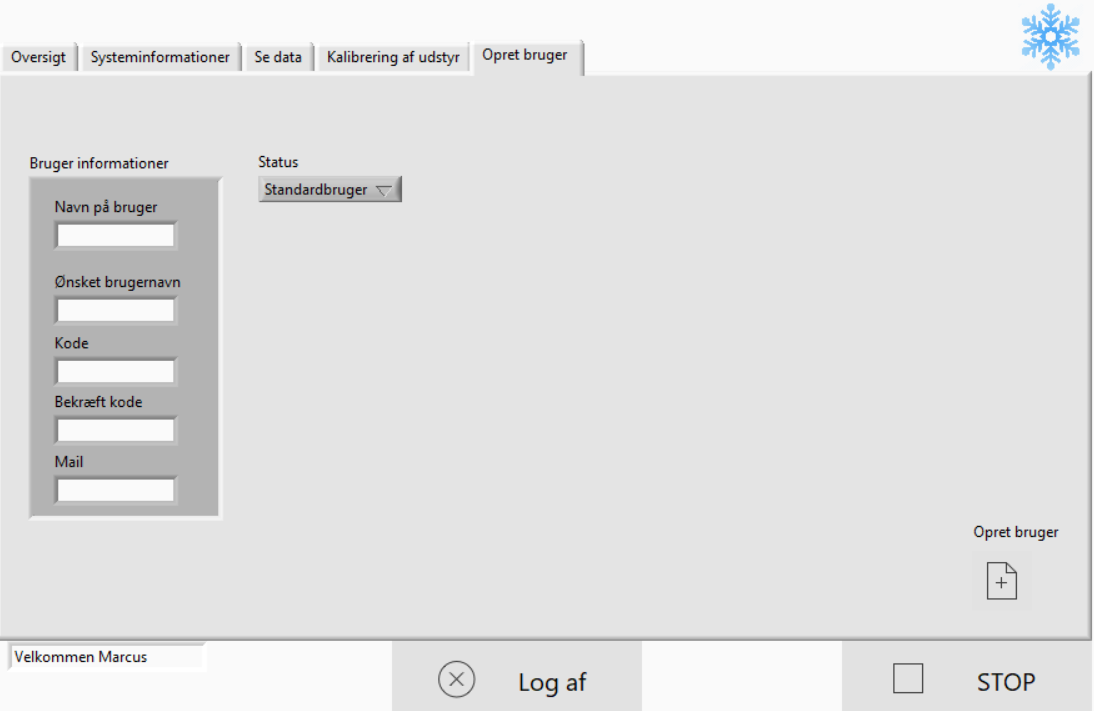
\includegraphics[width=0.80\textwidth]{Billeder/opret.png}
	\caption{\textit{Opret bruger}.}
	\label{fig:opret_bruger}
\end{figure}
%------------------------------------------------------------------------------
\section{Kalibrering (M.N. \& B.B.)}
Hvis brugeren er logget ind som administrator, er det muligt at tilgå de to kalibreringsprogrammer. Disse er ikke så visuelt udviklede som andre dele af programmet. Dette er ikke tænkt som værende nødvendigt, da det kun er administratorer, som kan tilgå disse kalibreringsprogrammer, og derfor vil de have en højere teknisk viden om programmet. Det antages derfor, at det ikke vil være nødvendigt med øvrige visuelle elementer, da administratorer allerede har kendskab til, hvordan programmet virker. \\
Programmerne kan ses afbildet i figur \ref{fig:FC_temp} og \ref{fig:FC_tryk}:
\begin{figure}[H]
	\centering
	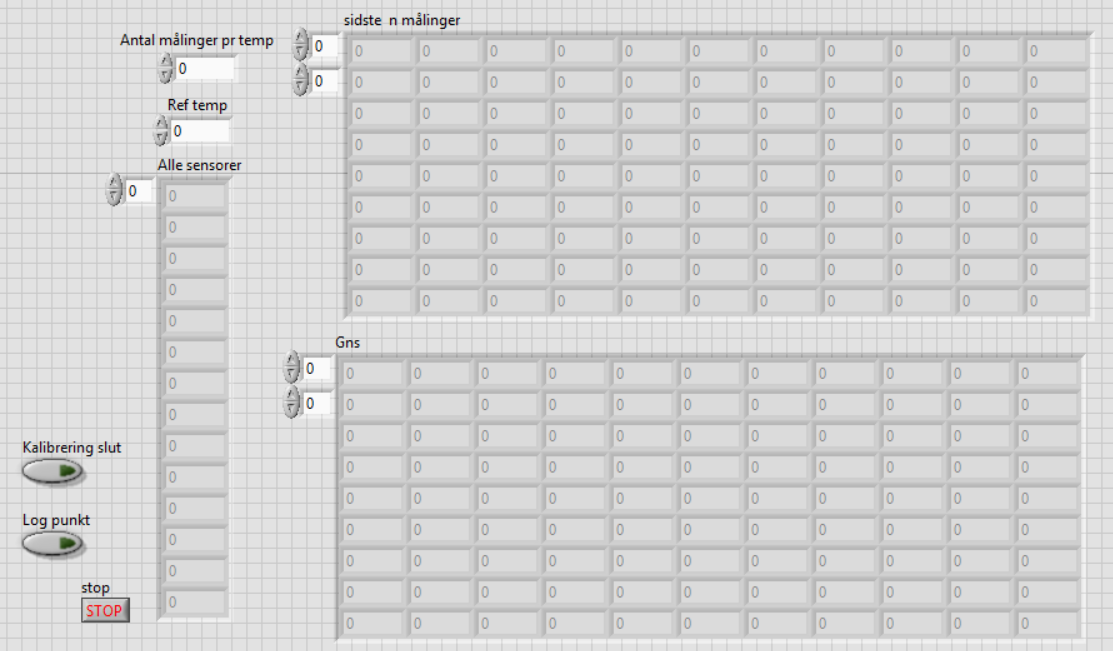
\includegraphics[width=0.80\textwidth]{Billeder/FCkali_termo.png}
	\caption{\textit{Forside til temperaturkalibrering}´.}
	\label{fig:FC_temp}
\end{figure}

\begin{figure}[H]
	\centering
	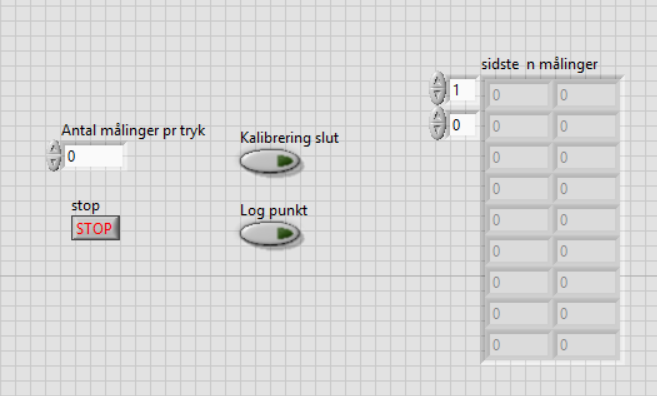
\includegraphics[width=0.80\textwidth]{Billeder/FCkali_tryk.png}
	\caption{\textit{Forside til trykkalibrering}.}
	\label{fig:FC_tryk}
\end{figure}
%------------------------------------------------------------------------------
\section{Styring (M.N. \& U.H.)}
Styringen af de forskellige komponenter i køleanlægget er en af vigtigste faktorer, når et køleanlæg skal køre. En af grundene til at styringen er så vigtig, er at køleanlægget skal fungere til bestemte formål. I dette tilfælde ønskes ikke en lavere temperatur end 3-4 \si{\celsius}, da temperaturer under dette kan resultere i, at mad- og drikkevarer fryser til. Dette vil dog kun forekomme, hvis kompressoren fortsætter med at køre på fuld kraft. Som følge at dette, vil det blive koldere og koldere i køleskabet, da kompressoren fortsat vil fjerne energi. 
%------------------------------------------------------------------------------
\subsection*{Styring af kompressor (M.N. \& U.H.)}
Kompressoren i det termodynamiske system er hovedkomponenten i kølekredsen. Denne kompressor indreguleres efter et setpunkt, som er bestemt af brugeren i den grafiske brugerflade (se afsnit \ref{sec:grafisk_bruger}). 
Selve kompressoren er en DC-kompressor, hvilket muliggør en regulering af omdrejningstallet, som også tidligere er nævnt i rapporten. Denne regulering gør, at kompressoren kan yde mindre i takt med at køleskabets temperatur kommer tættere på setpunktet. Omdrejningstallet bliver styret af en modstand fra 0 til 5000 \si{\Omega}, hvilket mere praktisk betyder, at når modstanden i kompressoren er 0 \si{\Omega}, kører den med 2500 RPM, mens den ved 5000 \si{\Omega} kører med 4000 RPM. 
Ud fra disse punkter laves en linære fremstilling for omdrejningstallet som funktion af modstanden, hvormed hældningstallet først findes:
\begin{align}
    a=\dfrac{\Delta Y}{\Delta X}=\dfrac{(4000-2500) \si{RPM}}{(5000-0) \si{\Omega}}=0,3
\end{align}
Startbetingelsen ved 0 \si{\Omega} kendes til $b=2500 \si{RPM}$, hvilket giver følgende linære fremstilling:
\begin{align}
    y(x)=a\cdot x + b \Leftrightarrow y(x)=0,3\cdot x + 2500
\end{align}
Ud fra den ovenstående ligning kan omdrejningstallet ved de forskellige modstande beregnes.\\
Kompressoren er foruden omdrejningsreguleringen også on/off-reguleret. Dette betyder, at når kompressoren har opnået den ønskede temperatur i køleskabet, slukkes den. Når der igen er behov for at køleskabet skal køles, tænder kompressoren igen. 
 %------------------------------------------------------------------------------
\subsection*{Styring af blæser (M.N. \& U.H.)}
Der er i køleskabet to blæsere, der sidder på hver sin varmeveksler. Blæserne har til formål at forøge effekten for varmevekslerne ved at tvinge en luftstrøm henover over disse. Dette medfører, at varmeovergangstallet stiger fra ca. \SI{10}{\frac{W}{m^2\cdot K}} ved fri konvektion til op mod \SI{100}{\frac{W}{m^2\cdot K}}, hvilket betyder, at der er behov for et mindre overfladeareal af varmeveksleren \ref{sec:bil_erfaringstal_U}. \\
Selve styringen af disse blæsere er relativ simpel, da disse er on/off-reguleret. Det vil sige, at enten er der ingen luftstrøm over en varmeveksler eller så er der en konstant luftstrøm. Blæseren på kondensatoren følger kompressorens on/off-regulering, hvilket betyder at blæseren på kondensatoren kører, når kompressoren er tændt, og ligeledes stopper, når kompressoren slukker. Grunden til at blæseren ikke fortsætter med at køre, når kompressoren stopper, er at der ikke er det samme behov for at fjerne varme. \\
Blæseren, der er placeret inden i køleskabet på fordamperen, kører konstant, da dette skaber en hurtigere og dermed mere effektiv nedkøling af drikkevarer. Det er dog ikke belejligt, at blæseren også kører, når køleskabsdøren åbnes, da den kolde luft herved blæses ud af køleskabet. Derfor er der på køleskabslågen sat en \textit{switch}, som slukker blæseren i køleskabet, når døren åbnes. 
%------------------------------------------------------------------------------
\section{Datalogning (M.N. \& U.H.)}
Udover at styre kompressoren har programmet også til formål at logge diverse værdier fra systemet. 
De forskellige målinger korrigeres først vha. en korrektionsværdi, hvorefter programmet logger de tidligere beskrevne tryk og temperaturer. Med hjælp fra dette, og en \textit{EES} makro \ref{sec:apndx_EES_makro}, kan LabVIEW sende de målte værdier til en tekstfil, som \textit{EES} kan læse. Efter \textit{EES} har læst disse værdier, udregnes størrelser af særlig interesse såsom entalpi, kuldeydelse, trykforhold samt COP, hvilket følger samme fremgangsmåde som i afsnit \ref{sec:indledendeberegninger}. 

Disse udregnede værdier skriver \textit{EES} til en anden tekstfil, som bliver læst af LabVIEW. Dette betyder, at LabVIEW hele tiden kan have udregnede størrelser alt efter hvilke tryk og temperature, som måles igennem systemet. 
Disse informationer logges løbende til en fil i et interval, som bestemmes af brugeren. 
%------------------------------------------------------------------------------
\end{document}